\documentclass{article}
\usepackage{tikz}
\usetikzlibrary{decorations.pathreplacing}
\usepackage{amsmath}

\begin{document}

\vspace{-200pt}

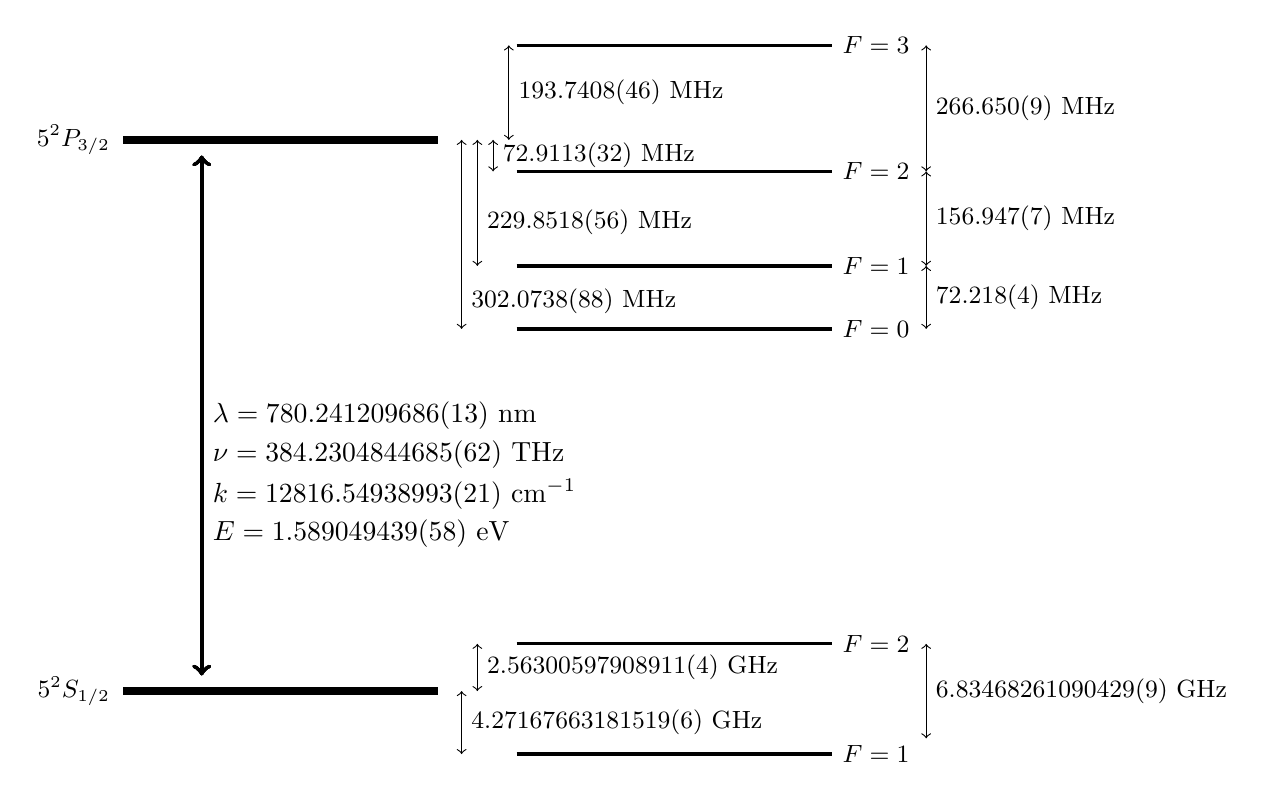
\begin{tikzpicture}[scale=2]

% rb 87
% lower level: 5s 1/2
\draw[line width=1mm] (-3,0) -- (-1,0) node[left, xshift=-4cm] {\small $5^2S_{1/2}$};
\draw[very thick] (-0.5,0.3) -- (1.5,0.3) node[right] {\small $F = 2$};
\draw[very thick] (-0.5,-0.4) -- (1.5,-0.4) node[right] {\small $F = 1$};

% annotate hfs for 5s: F=1 to F=2
\draw[<->] (2.1,0.3) -- (2.1,-0.3) node[midway,right] {\small $6.83468261090429(9)~\text{GHz}$}; % 1 to 2

% annotate hfs for 5s: ground state to F=1,2
\draw[<->] (-0.85,0) -- (-0.85,-0.4) node[midway,right] {\small $4.27167663181519(6)~\text{GHz}$}; % to 1
\draw[<->] (-0.75,0) -- (-0.75,0.3) node[midway,right] {\small $2.56300597908911(4)~\text{GHz}$}; % to 2


% upper level: 5p 3/2
\draw[line width=1mm] (-3,3.5) -- (-1,3.5) node[left, xshift=-4cm] {\small $5^2P_{3/2}$};

\draw[very thick] (-0.5,4.1) -- (1.5,4.1) node[right] {\small $F = 3$};
\draw[very thick] (-0.5,3.3) -- (1.5,3.3) node[right] {\small $F = 2$};
\draw[very thick] (-0.5,2.7) -- (1.5,2.7) node[right] {\small $F = 1$};
\draw[very thick] (-0.5,2.3) -- (1.5,2.3) node[right] {\small $F = 0$};

% annotate hfs for 5p: each F state to other F state 
\draw[<->] (2.1,2.3) -- (2.1,2.7) node[midway,right] {\small $72.218(4)~\text{MHz}$}; %0 to 1
\draw[<->] (2.1,2.7) -- (2.1,3.3) node[midway,right] {\small $156.947(7)~\text{MHz}$}; % 1 to 2
\draw[<->] (2.1,3.3) -- (2.1,4.1) node[midway,right] {\small $266.650(9)~\text{MHz}$}; % 2 to 3

% annotate hfs for 5p: ground state to each F state 
\draw[<->] (-0.85,3.5) -- (-0.85,2.3) node[below, right, yshift = 0.35cm] {\small $302.0738(88)~\text{MHz}$};
\draw[<->] (-0.75,3.5) -- (-0.75,2.7) node[below, right, yshift = 0.55cm] {\small $229.8518(56)~\text{MHz}$};
\draw[<->] (-0.65,3.5) -- (-0.65,3.3) node[midway,right] {\small $72.9113(32)~\text{MHz}$};
\draw[<->] (-0.55,3.5) -- (-0.55,4.1) node[midway,right] {\small $193.7408(46)~\text{MHz}$};


% % cooling transition
% \draw[dashed] (-0.5,4.0) -- (1.5,4.0) node[right] {};
% % \draw[->,thick, color = red] (1,0.3) -- (1,4.0) node[midway, left, xshift=-0.2cm] {\small $780.241~\text{nm}$};
% \draw[->,thick, color = red] (1.0,0.3) -- (1.0,4.0) node[midway, left, yshift = -1.2cm] {Cooling};


% % repump transition
% \draw[dashed] (-0.5,3.0) -- (1.5,3.0) node[right] {};
% % \draw[->,thick, color = red] (1,0.3) -- (1,4.0) node[midway, left, xshift=-0.2cm] {\small $780.241~\text{nm}$};
% \draw[->,thick, color = brown] (1.3,-0.4) -- (1.3,3.0) node[midway, right, yshift = 0.5cm] {Repump};


% % transitions
% \draw[dashed] (-0.5,3.0) -- (1.5,3.0) node[right] {};
% % \draw[->,thick, color = red] (1,0.3) -- (1,4.0) node[midway, left, xshift=-0.2cm] {\small $780.241~\text{nm}$};
% \draw[->,thick, color = brown] (1.3,-0.4) -- (1.3,3.0) node[midway, right, yshift = 0.5cm] {Repump};


% annotate fs info
\draw[<->, line width = 0.5mm] (-2.5,0.1) -- (-2.5,3.4) node[midway,right, yshift = 0.0cm] {$\lambda = 780.241209686(13)~\text{nm}$};
\draw[<->, line width = 0.5mm] (-2.5,0.1) -- (-2.5,3.4) node[midway,right, yshift = -0.5cm] {$\nu = 384.2304844685(62)~\text{THz}$};
\draw[<->, line width = 0.5mm] (-2.5,0.1) -- (-2.5,3.4) node[midway,right, yshift = -1.0cm] {$k = 12816.54938993(21)~\text{cm$^{-1}$}$};
\draw[<->, line width = 0.5mm] (-2.5,0.1) -- (-2.5,3.4) node[midway,right, yshift = -1.5cm] {$E = 1.589049439(58)~\text{eV}$};

\end{tikzpicture}

\vspace{10pt}

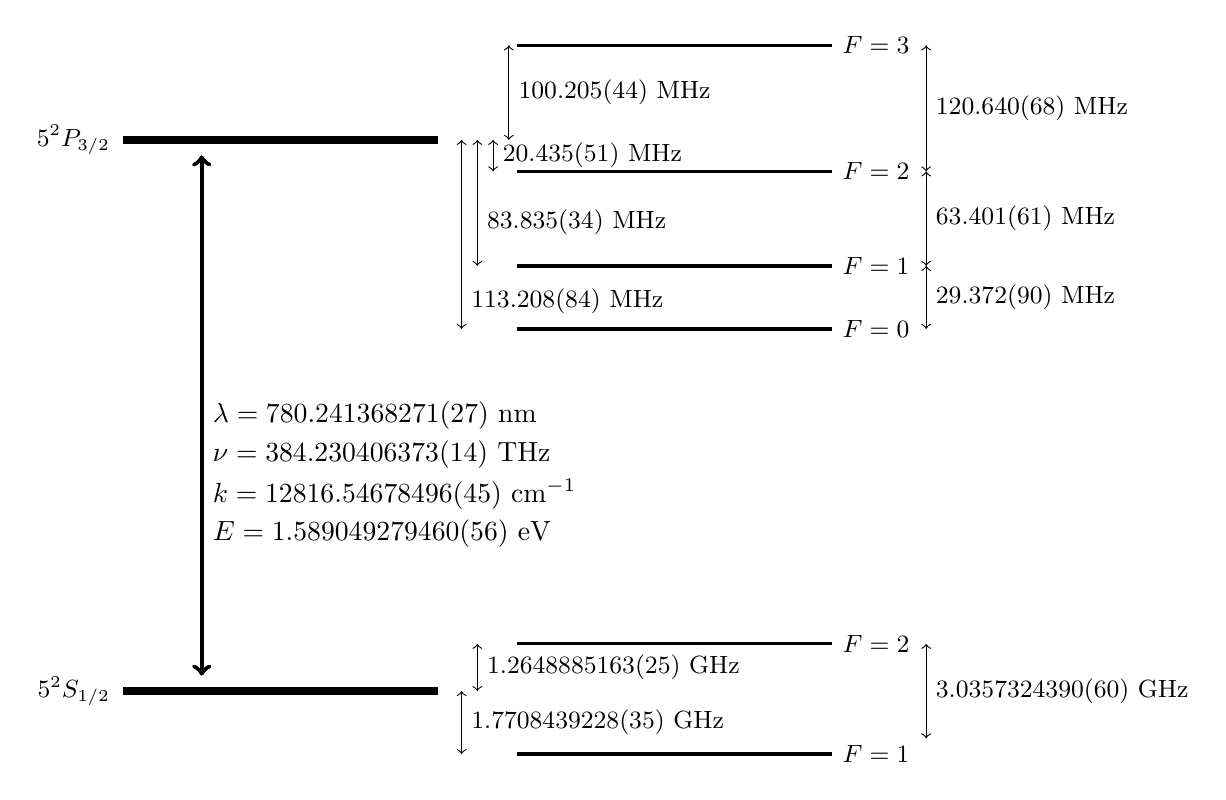
\begin{tikzpicture}[scale=2]

% rb 85
% lower level: 5s 1/2
\draw[line width=1mm] (-3,0) -- (-1,0) node[left, xshift=-4cm] {\small $5^2S_{1/2}$};
\draw[very thick] (-0.5,0.3) -- (1.5,0.3) node[right] {\small $F = 2$};
\draw[very thick] (-0.5,-0.4) -- (1.5,-0.4) node[right] {\small $F = 1$};

% annotate hfs for 5s: F=1 to F=2
\draw[<->] (2.1,0.3) -- (2.1,-0.3) node[midway,right] {\small $3.0357324390(60)~\text{GHz}$}; % 1 to 2

% annotate hfs for 5s: ground state to F=1,2
\draw[<->] (-0.85,0) -- (-0.85,-0.4) node[midway,right] {\small $1.7708439228(35)~\text{GHz}$}; % to 1
\draw[<->] (-0.75,0) -- (-0.75,0.3) node[midway,right] {\small $1.2648885163(25)~\text{GHz}$}; % to 2


% upper level: 5p 3/2
\draw[line width=1mm] (-3,3.5) -- (-1,3.5) node[left, xshift=-4cm] {\small $5^2P_{3/2}$};

\draw[very thick] (-0.5,4.1) -- (1.5,4.1) node[right] {\small $F = 3$};
\draw[very thick] (-0.5,3.3) -- (1.5,3.3) node[right] {\small $F = 2$};
\draw[very thick] (-0.5,2.7) -- (1.5,2.7) node[right] {\small $F = 1$};
\draw[very thick] (-0.5,2.3) -- (1.5,2.3) node[right] {\small $F = 0$};

% annotate hfs for 5p: each F state to other F state 
\draw[<->] (2.1,2.3) -- (2.1,2.7) node[midway,right] {\small $29.372(90)~\text{MHz}$}; %1 to 2
\draw[<->] (2.1,2.7) -- (2.1,3.3) node[midway,right] {\small $63.401(61)~\text{MHz}$}; % 2 to 3
\draw[<->] (2.1,3.3) -- (2.1,4.1) node[midway,right] {\small $120.640(68)~\text{MHz}$}; % 3 to 4

% annotate hfs for 5p: ground state to each F state 
\draw[<->] (-0.85,3.5) -- (-0.85,2.3) node[below, right, yshift = 0.35cm] {\small $113.208(84)~\text{MHz}$};
\draw[<->] (-0.75,3.5) -- (-0.75,2.7) node[below, right, yshift = 0.55cm] {\small $83.835(34)~\text{MHz}$};
\draw[<->] (-0.65,3.5) -- (-0.65,3.3) node[midway,right] {\small $20.435(51)~\text{MHz}$};
\draw[<->] (-0.55,3.5) -- (-0.55,4.1) node[midway,right] {\small $100.205(44)~\text{MHz}$};


% % cooling transition
% \draw[dashed] (-0.5,4.0) -- (1.5,4.0) node[right] {};
% % \draw[->,thick, color = red] (1,0.3) -- (1,4.0) node[midway, left, xshift=-0.2cm] {\small $780.241~\text{nm}$};
% \draw[->,thick, color = red] (1.0,0.3) -- (1.0,4.0) node[midway, left, yshift = -1.2cm] {Cooling};


% % repump transition
% \draw[dashed] (-0.5,3.0) -- (1.5,3.0) node[right] {};
% % \draw[->,thick, color = red] (1,0.3) -- (1,4.0) node[midway, left, xshift=-0.2cm] {\small $780.241~\text{nm}$};
% \draw[->,thick, color = brown] (1.3,-0.4) -- (1.3,3.0) node[midway, right, yshift = 0.5cm] {Repump};



% annotate fs info
\draw[<->, line width = 0.5mm] (-2.5,0.1) -- (-2.5,3.4) node[midway,right, yshift = 0.0cm] {$\lambda = 780.241368271(27)~\text{nm}$};
\draw[<->, line width = 0.5mm] (-2.5,0.1) -- (-2.5,3.4) node[midway,right, yshift = -0.5cm] {$\nu = 384.230406373(14)~\text{THz}$};
\draw[<->, line width = 0.5mm] (-2.5,0.1) -- (-2.5,3.4) node[midway,right, yshift = -1.0cm] {$k = 12816.54678496(45)~\text{cm$^{-1}$}$};
\draw[<->, line width = 0.5mm] (-2.5,0.1) -- (-2.5,3.4) node[midway,right, yshift = -1.5cm] {$E = 1.589049279460(56)~\text{eV}$};


\end{tikzpicture}

\end{document}
